\documentclass{article}

\usepackage{babel}
\usepackage{blindtext}
\usepackage{caption}
\usepackage{graphicx}

\author{Ee Xuan Tan (4907531) \and Elvira Voorneveld (4930975) \and William Narchi (5046122)}
\date{Group 40}
\title{Computer Graphics Project}

\begin{document}
    \maketitle

    \section{Work Distribution}
    \begin{tabular}{ |p{2.5cm}||p{2.5cm}|p{2.5cm}|p{2.5cm}| }
        \hline
        \textbf{Feature} &\textbf{Ee Xuan} &\textbf{Elvira} &\textbf{William}\\
        \hline
        Shading                        &0\%    &100\%  &0\%\\
        Recursion                      &0\%    &0\%    &100\%\\
        Hard Shadows                   &0\%    &100\%  &0\%\\
        Soft Shadows                   &100\%  &0\%    &0\%\\
        BVH                            &40\%   &20\%   &40\%\\
        Interpolation                  &0\%    &100\%  &0\%\\
        Planar Area                    &100\%  &0\%    &0\%\\
        Bloom Filter                   &0\%    &0\%    &100\%\\
        Anti-aliasing                  &0\%    &0\%    &100\%\\
        Multiple rays                  &0\%    &0\%    &100\%\\
        Depth of Field                 &0\%    &0\%    &100\%\\
        \hline
    \end{tabular}

    \newpage

    \section{Features}
    \subsection{Main Requirements}
    \subsubsection{Phong Shading}
    At each intersection point, the diffuse and specular terms from the Phong Model are used to calculate the 
    lighting. We ignore the ambient term, as it is a crude approximation of global illumination, and therefore 
    not necessary to incorporate. First, the lighting is computed separately for every light source in the 
    scene, and those results are then added together to compute the final, direct illumination.

    \begin{center}
        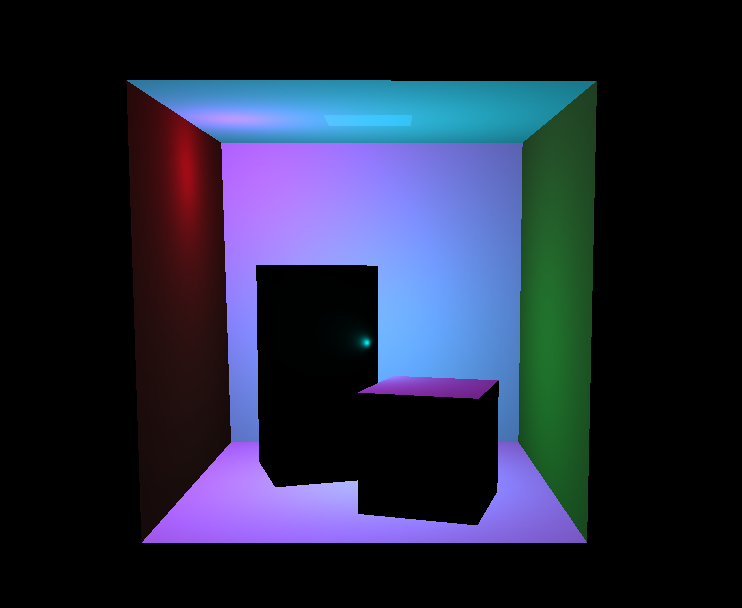
\includegraphics[scale=0.39]{images/phong_shading_showcase}

        The lighting effects produced by phong shading with two light sources RGB(255, 0, 255) and RGB(0, 255, 255)

        \vspace{5mm}

        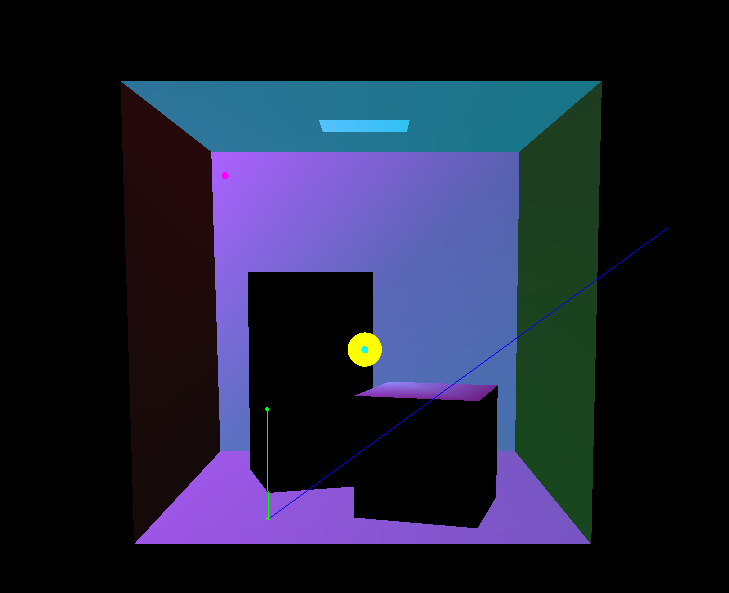
\includegraphics[scale=0.40]{images/phong_shading_debug}

        The phong shading debug, showing one ray shot from another angle, along with its normal
    \end{center}

    \newpage

    \subsubsection{Recursive Ray Tracing}
    The recursive ray tracer builds upon the previously implemented ray shading,
    creating reflection rays at each intersection point and adding the value of the reflection ray's lighting 
    to the initial ray's specular component, provided that the intersection point is on a specular surface 
    and that the reflected ray intersects a surface. This is done recursively until one of the previously 
    mentioned limiting conditions applies or the recursion depth reaches a pre-set \emph{RECURSION\_LIMT}.

    \begin{center}
        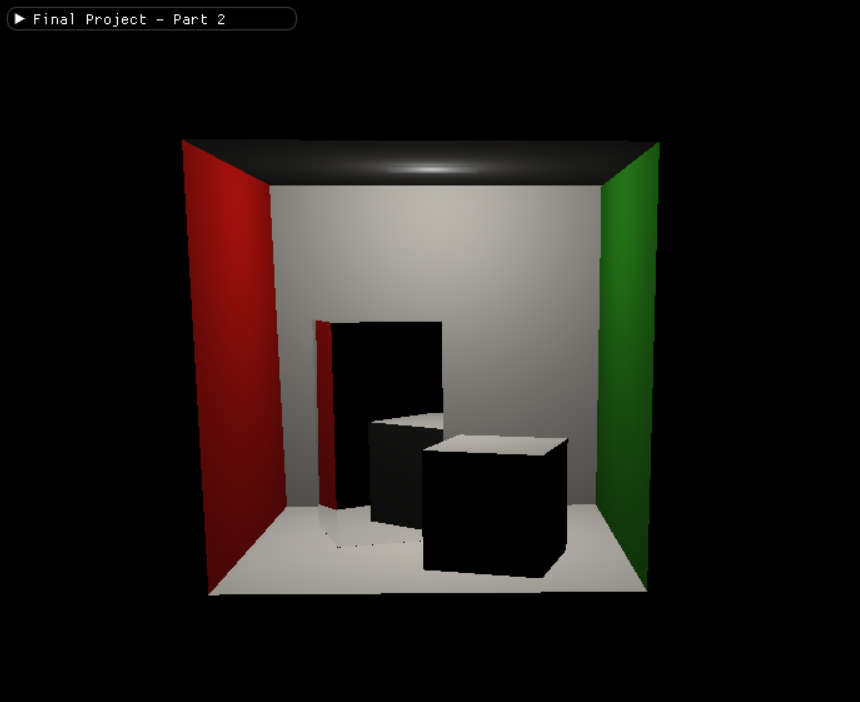
\includegraphics[scale=0.45]{images/recursive_ray_tracer_showcase}

        The complex specular effects produced by recursive ray tracing, which include proper mirror simulation

        \vspace{5mm}

        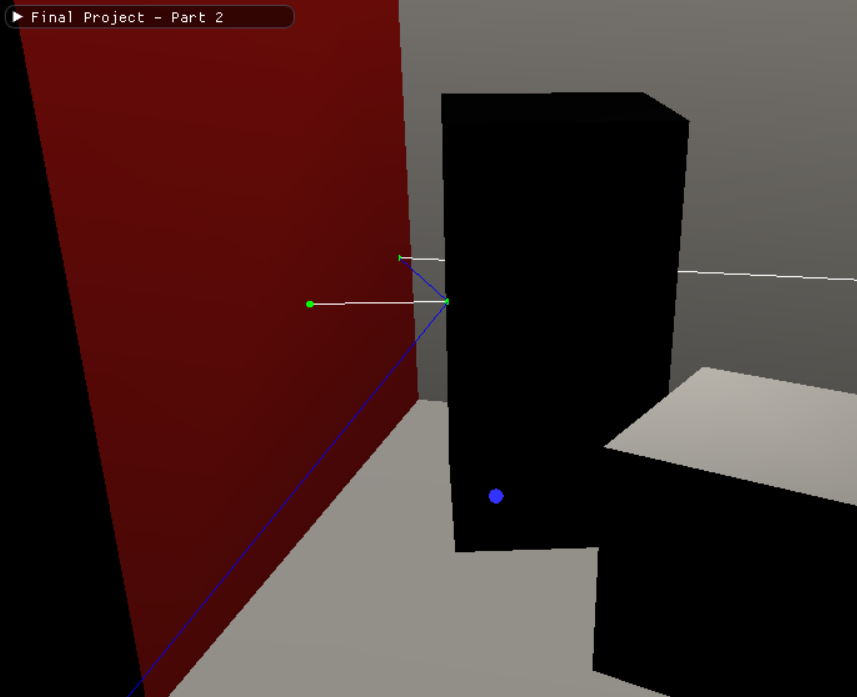
\includegraphics[scale=0.45]{images/recursive_ray_tracer_debug}

        The recursive ray tracer debug, showing two total rays in the recursive chain, along with their normals
    \end{center}

    \newpage

    \subsubsection{Hard Shadows}
    To discover which light source(s) contribute to the lighting of a certain point, ray(s) are shot from the 
    intersection point towards the light source(s). For each light source, it is computed whether or not there 
    is a direct path between the intersection point and the respective light source. Only point lights that 
    directly shine upon the intersection point will be considered when computing the lighting in that area,
    leaving it black if none of the point lights contribute.

    \begin{center}
        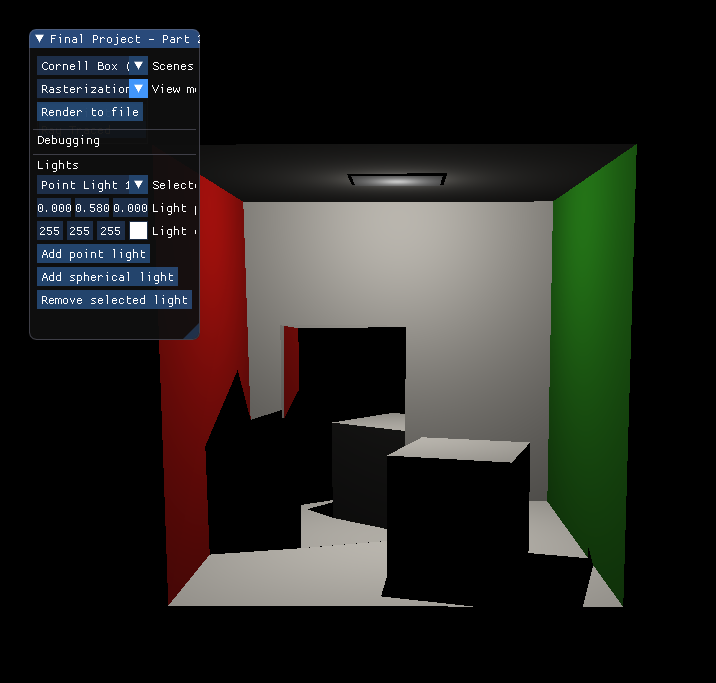
\includegraphics[scale=0.365]{images/hard_shadow_showcase}

        The result of using a single point light source to create hard shadows.

        \vspace{5mm}

        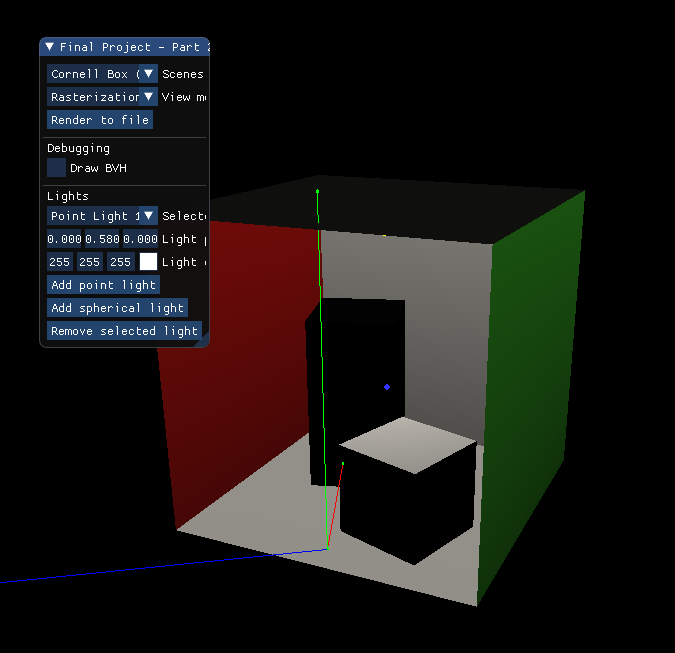
\includegraphics[scale=0.39]{images/hard_shadow_debug}

        The hard shadow debug, showing a ray shot from another angle, along with its normal and a red line 
        indicating the intersection with another object before reaching the point light source.
    \end{center}

    \newpage

    \subsubsection{Soft Shadows}
    It first generates uniformly distributed rays from the spherical light source using the fibonacci sequence 
    with a golden ratio to ensure equal step sizes. To prevent light rays from the opposite side of the sphere 
    to influence the intersection point, the center and radius of the sphere are used to calculate the longest 
    a light ray on the appropriate side could be. A pre-determined number of sample points is taken and used 
    to see if they do not intersect with an object before reaching the intersection point. Once this is 
    established, we enumerate the samples that reached the point and divide it by the total amount of rays 
    shot from the spherical light source, resulting in the light value at that point.

    \begin{center}
        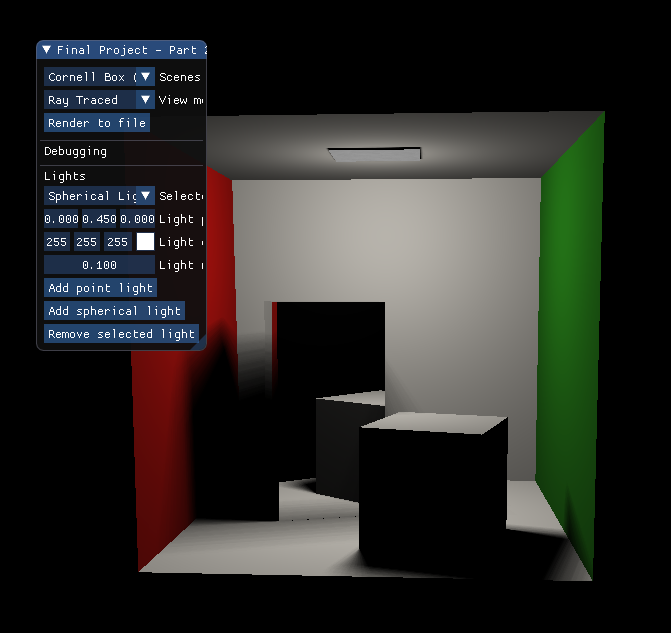
\includegraphics[scale=0.41]{images/soft_shadow_showcase}

        The result of using a single spherical light source with the \emph{SPHERE\_SAMPLE\_LIMIT} set to 100 
        to create soft shadows.

        \vspace{5mm}

        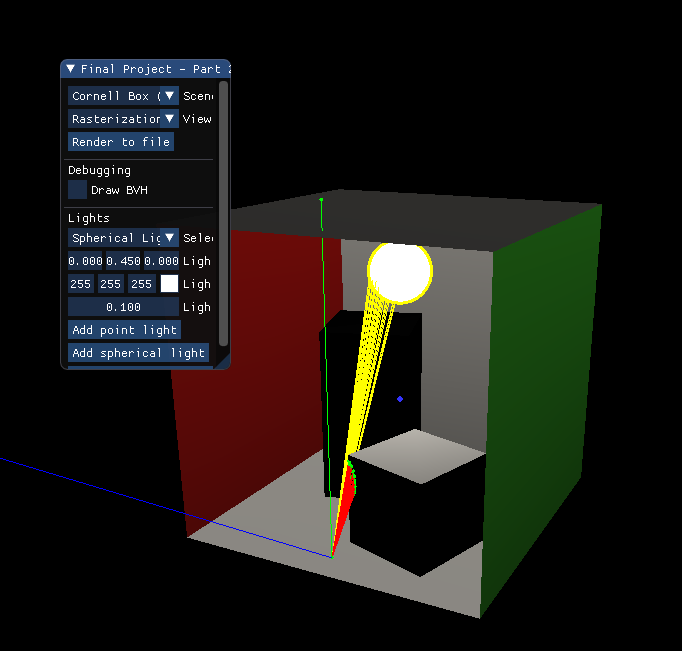
\includegraphics[scale=0.41]{images/soft_shadow_debug}

        The soft shadow debug, showing all of the uniformly distributed samples generated by the spherical 
        light source. The yellow lines indicate a direct path from the intersection to the light source and 
        the red lines indicate the intersection with another object before reaching the spherical light source.
    \end{center}

    \newpage

    \subsubsection{Bounding Volume Hierarchy}
    This BVH is contructed using the SAH and binning. It starts off by indexing every triangle in the model 
    and creating the first AABB that contains all of the triangles. It then proceeds to split this bounding 
    box until the maximum level or the minimum amount of triangles is reached. Splitting relies on the use of 
    alternating axes and bins to create a split boundary. The longest axis in the bounding box being analysed 
    is determined and used for the split boundary. It goes on to compute the cost function of these new 
    splits, and only creates new nodes for them if they are more efficient to use than the original. After 
    constructing the BVH, it will recursively check if a ray shot at the scene will intersect with the parent 
    AABB or any of its children. If there is no intersection with any of the leaf nodes, there is no intersection 
    with the model. Otherwise, all triangles in the respective leaf node will be checked for intersection. Two 
    constructors are provided for the BVH: one where the maximum tree depth can be manually set; and one where 
    the number of triangles in the scene is used as a heuristic to determine the maximum tree depth.

    \begin{figure}[!htb]
        \minipage{0.48\textwidth}
          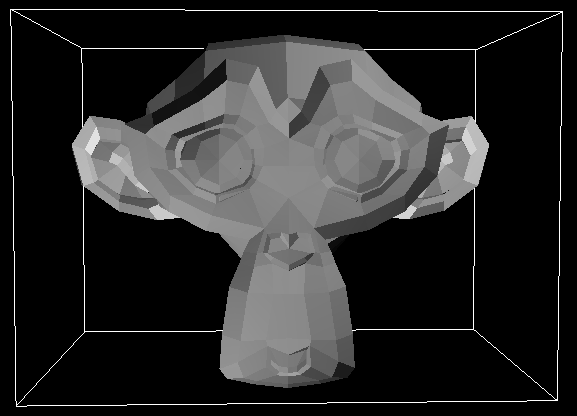
\includegraphics[width=\linewidth, height=4.7cm]{images/bvh_level_one}
          \caption*{The first level of the BVH}
        \endminipage\hfill
        \minipage{0.48\textwidth}
          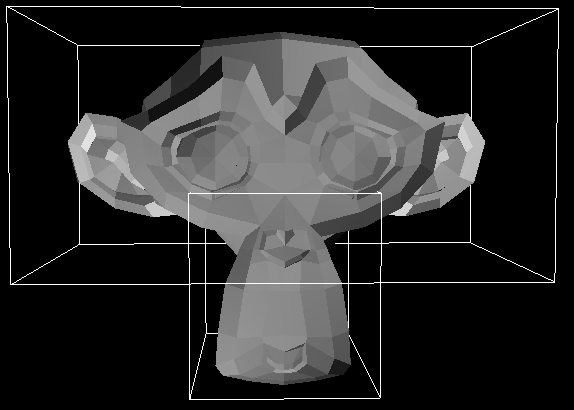
\includegraphics[width=\linewidth, height=4.7cm]{images/bvh_level_two}
          \caption*{The second level of the BVH}
        \endminipage
      \end{figure}
      
      \begin{figure}[!htb]
        \minipage{0.48\textwidth}
          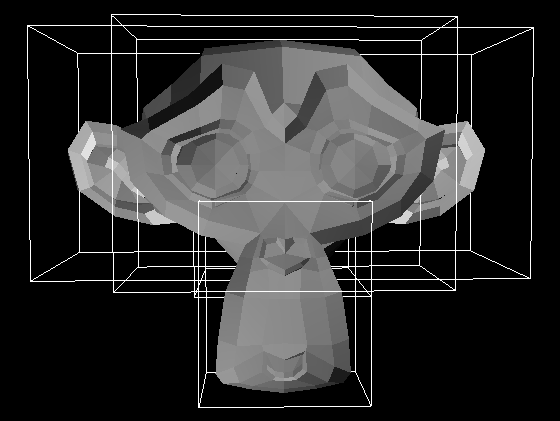
\includegraphics[width=\linewidth, height=4.7cm]{images/bvh_level_three}
          \caption*{The third level of the BVH}
        \endminipage\hfill
        \minipage{0.48\textwidth}
          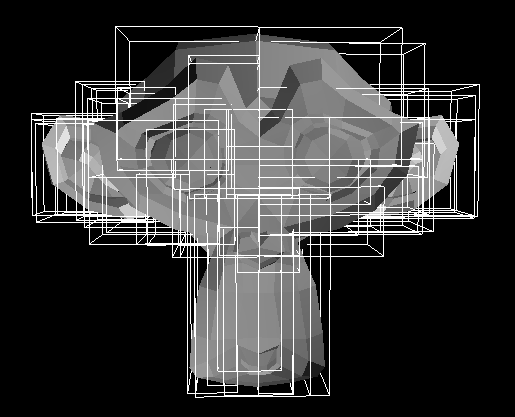
\includegraphics[width=\linewidth, height=4.7cm]{images/bvh_level_ten}
          \caption*{The tenth level of the BVH}
        \endminipage
    \end{figure}

    \newpage

    \subsection{Extra Requirements}
    \subsubsection{Interpolation}
    A simple method for computing interpolated values. When a ray hits a triangle, the alpha, beta and gamma 
    values for the barycentric coordinates are calculated using the triangle areas. Those coordinates are 
    used in combination with the vertex normals to compute the new and improved triangle normal.

    \begin{figure}[!htb]
      \centering
      \captionsetup{justification=centering}
      \minipage{0.49\textwidth}
        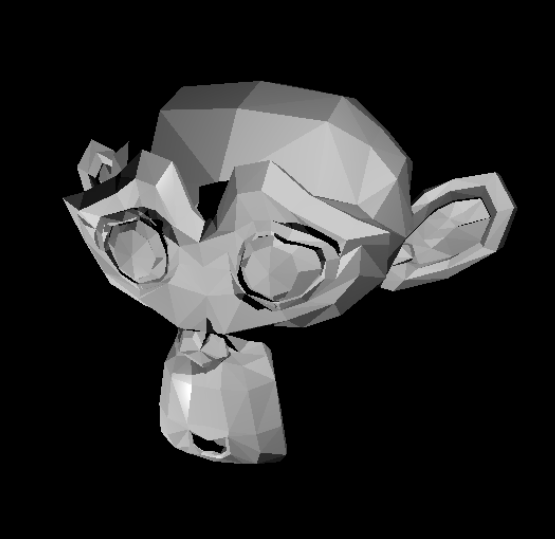
\includegraphics[width=\linewidth, height=6cm]{images/monke_no_bary}
        \caption*{Monkey without interpolation}
      \endminipage\hfill
      \minipage{0.49\textwidth}
        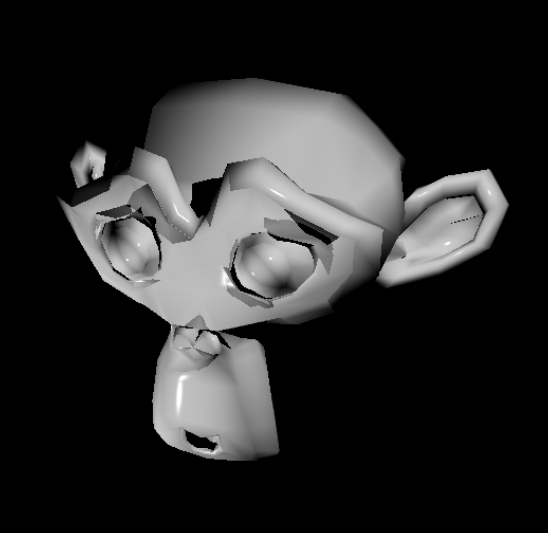
\includegraphics[width=\linewidth, height=6cm]{images/monke_bary}
        \caption*{Monkey with interpolation}
      \endminipage
      \vspace{5mm}
      \minipage{0.49\textwidth}
        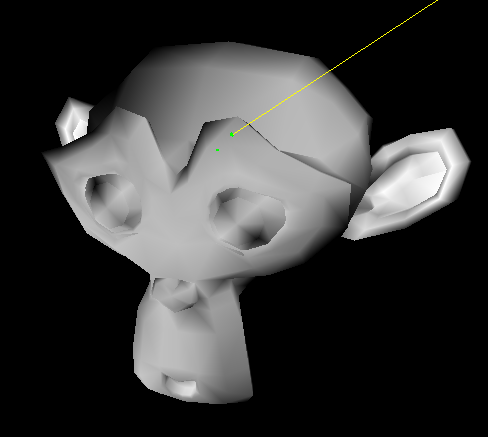
\includegraphics[width=\linewidth, height=6cm]{images/monke_no_bary_debug}
        \caption*{Debug without interpolation, the green normal is very small}
      \endminipage\hfill
      \minipage{0.49\textwidth}
        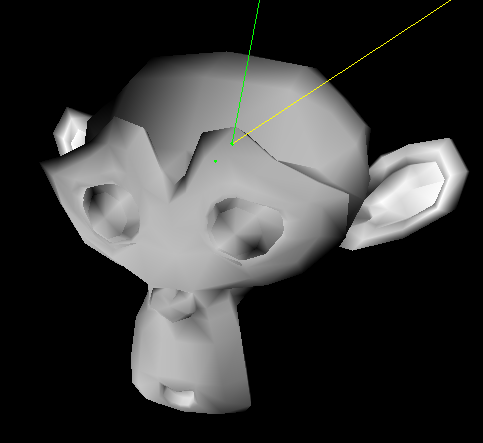
\includegraphics[width=\linewidth, height=6cm]{images/monke_bary_debug}
        \caption*{Debug with interpolation, the green normal is appropriately sized}
      \endminipage
    \end{figure}

    \subsubsection{Planar Area Light}
    To be constructed

    \subsubsection{Bloom Filter}
    A simple bloom filter that uses a box blur filter for the underlying blurring. It functions very similarly 
    to what was described in the slides for lecture 3, in that it culls pixels below a particular threshold 
    and applies the box filter implementation described in the slides onto the filtered pixels, before adding 
    the result to the un-processed pixel values. Due to the flatness of the available scenes' colour range,
    the bloom filter looks slightly exaggerated.

    \begin{figure}[!htb]
        \minipage{0.49\textwidth}
          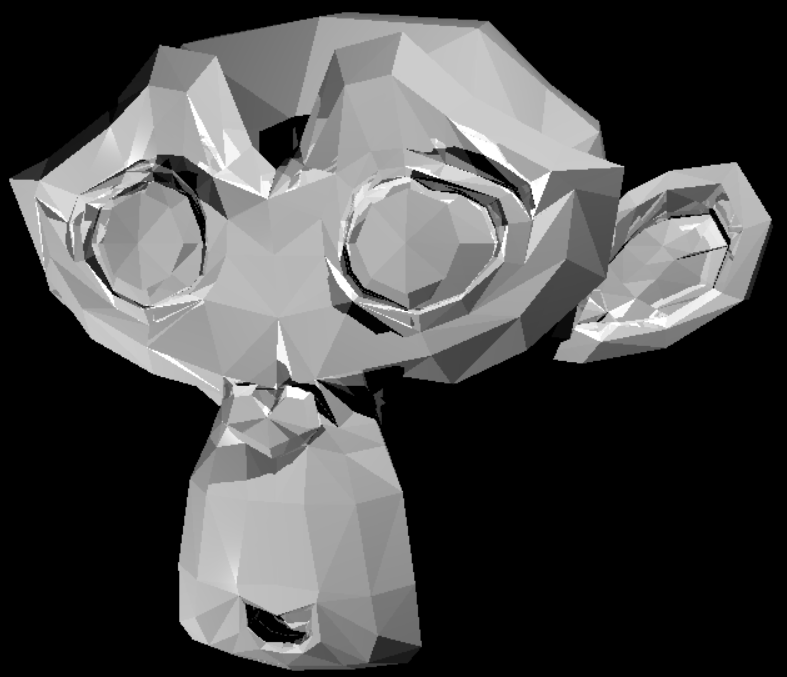
\includegraphics[width=\linewidth, height=5.5cm]{images/monkey_no_bloom}
          \caption*{Monkey without bloom}
        \endminipage\hfill
        \minipage{0.49\textwidth}
          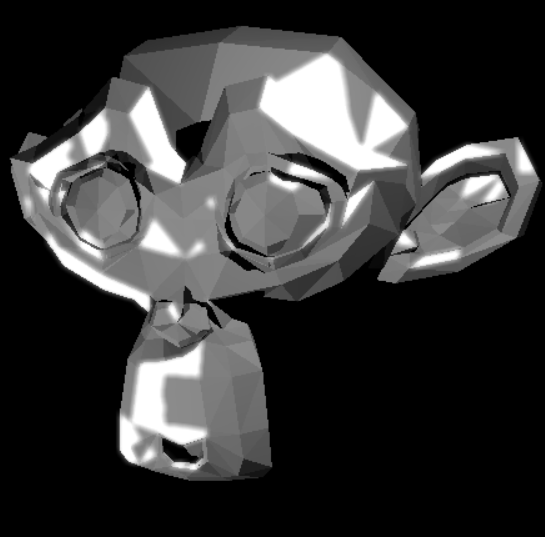
\includegraphics[width=\linewidth, height=5.5cm]{images/monkey_bloom}
          \caption*{Monkey with bloom filter applied}
        \endminipage
    \end{figure}
    
    \subsubsection{Cast Multiple Rays Per Pixel / Anti-Aliasing}
    A simple super-sampling anti-aliasing method that renders multiple rays per pixel (in effect, rendering 
    at a higher resolution) using a uniform distribution of samples. The colour values of the sample rays are 
    then averaged with no weighting to produce the final colour value. The exact degree of super-sampling can 
    be adjusted via the \emph{SAMPLING\_FACTOR} variable. As can clearly be seen in the figure below, the end 
    result is a much smoother image, with far fewer visible jagged edges and higher overall fidelity.

    \begin{figure}[!htb]
        \minipage{0.49\textwidth}
          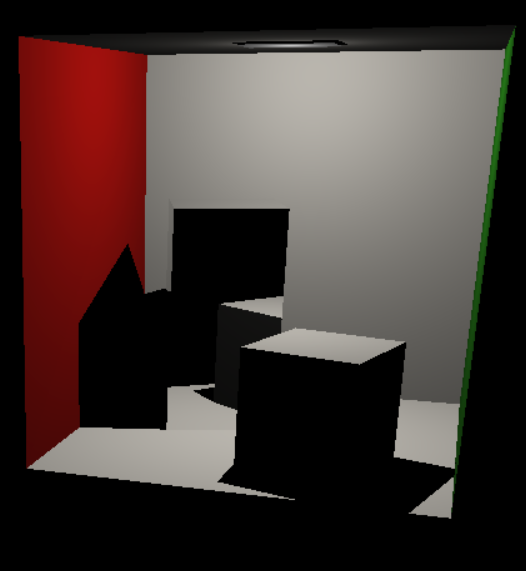
\includegraphics[width=\linewidth, height=6cm]{images/supersampling_non_supersampled}
          \caption*{Render without super-sampling}
        \endminipage\hfill
        \minipage{0.49\textwidth}
          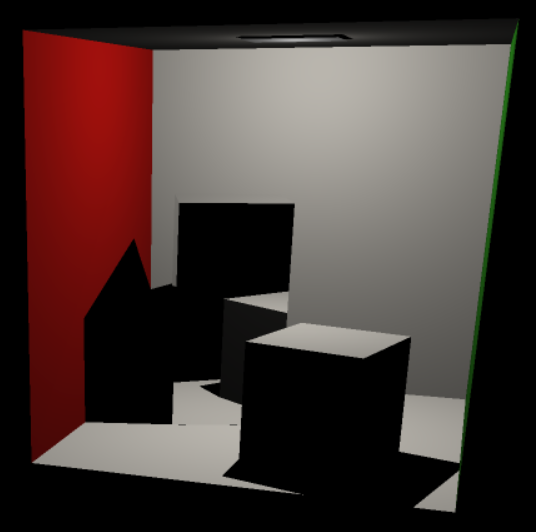
\includegraphics[width=\linewidth, height=6cm]{images/supersampling_supersampled}
          \caption*{Render with 2x super-sampling}
        \endminipage
    \end{figure}

    \begin{center}
      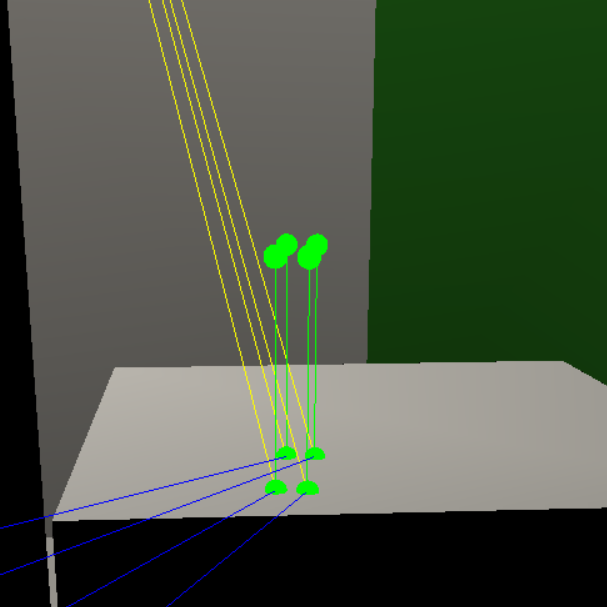
\includegraphics[scale=0.75]{images/supersampling_debugger.png}

      Visual debug at a 2x super-sampling ratio showing 4 rays in total (rays are projected from a far 
      distance for easier demonstration)
    \end{center}

    \subsubsection{Depth of Field}
    A post-processing depth of field filter that attempts to emulate real-life cameras. It works by first
    creating a depth buffer using the \emph{t} values and vector components of the camera rays, and then computing an
    average depth value of an adjustable sampling 'box' at the center of the viewport. This value is then
    used as the mean value of a normal (Gaussian) distribution, and the standard deviation of all valid
    pixels (ones whose rays interesected with an object) is computed and used as the standard deviation
    for the distribution. A box blur filter is applied on all of the pixels in the viewport and then
    the depth value of each pixel is input into the probability density function of the normal distribution
    established earlier. The output is used to compute the blend between the blurred and sharp pixel values,
    effectively allowing variable blurring depending on the depth of each pixel compared to the 'focal point',
    which is the average value computed from earlier. The size of the underlying blur filter, the number of
    pixels used as samples for the 'focal point' and a skew to arbitrarily strengthen or weaken the applied blurred
    are all adjustable.

    \begin{figure}[!htb]
      \minipage{0.49\textwidth}
        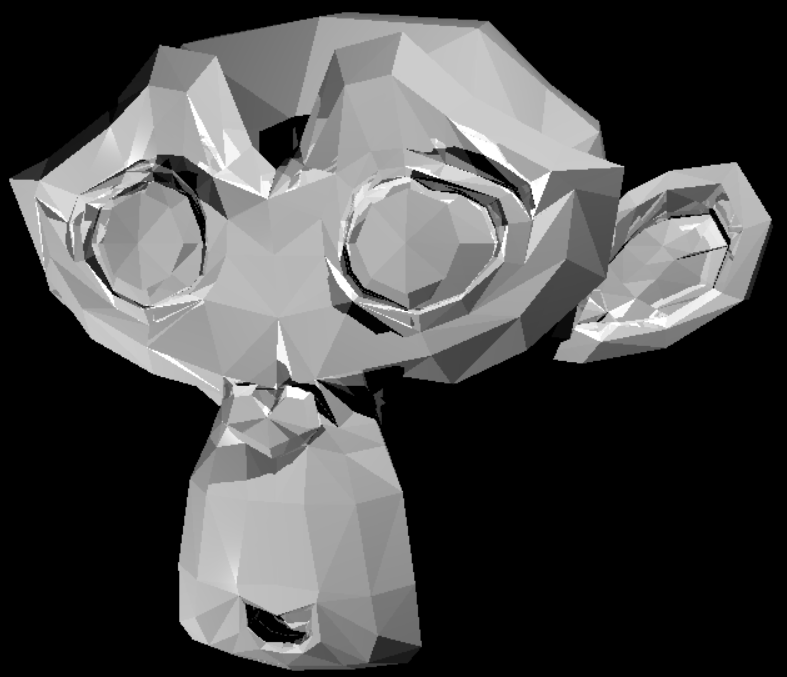
\includegraphics[width=\linewidth, height=6cm]{images/monkey_no_bloom}
        \caption*{Normal monkey render}
      \endminipage\hfill
      \minipage{0.49\textwidth}
        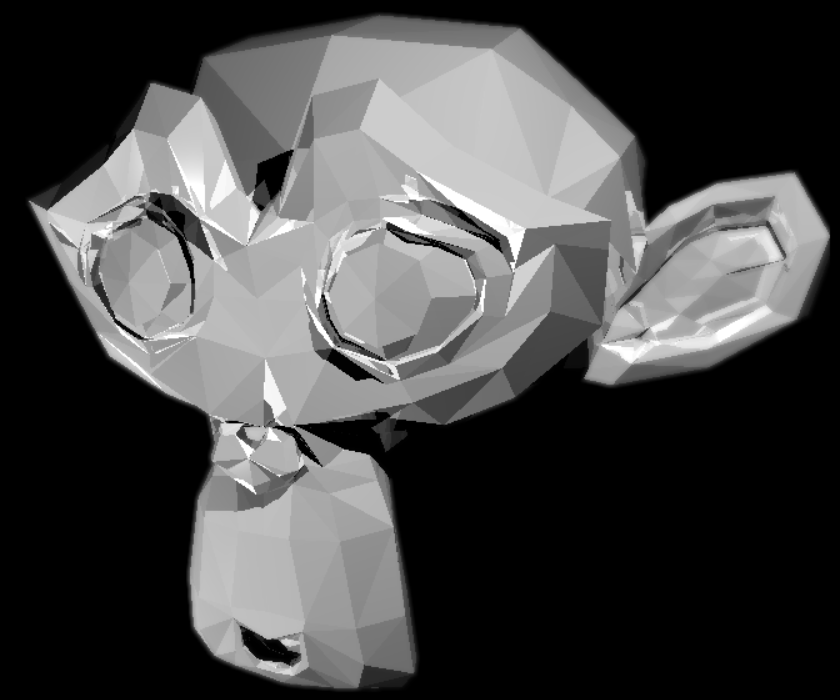
\includegraphics[width=\linewidth, height=6cm]{images/monkey_dof}
        \caption*{Monkey render with depth of field filter}
      \endminipage
  \end{figure}

  The effect is particularly noticeable on the back of the monkey's head and its ears, which receive a substantial amount
  of blur due to being relatively far from the 'focal point'.

    \newpage

    \section{Models}
    No extra models were used.

    \section{Performance Test}
    The following table shows the number of triangles contained in a scene, the time it took to render that 
    scene without the extra features, with the extra features, and the amount of BVH levels that were 
    constructed ().
    
    \vspace{5mm}
    
    \noindent\begin{tabular}{ |p{2.8cm}||p{1.6cm}|p{1.6cm}|p{1.6cm}|p{1.6cm}| }
      \hline
      \textbf{Feature} &\textbf{Cube} &\textbf{Cornell} &\textbf{Monkey} &\textbf{Dragon}\\
      \hline
      Number Triangles  &12     &32     &968    &87130\\
      Render Time       &0s     &0s     &0s     &0s\\
      Extra Time        &0s     &0s     &0s     &0s\\
      BVH Levels        &0      &0      &0      &0\\
      \hline
    \end{tabular}
\end{document}
